%This file can be compiled by as a standalone document 
%the preamble will be imported from the main file
%%
\documentclass[../main.tex]{subfiles} 
%../main.tex is the path to the main file

\begin{document} 
%Everything below this point will appear in the main document

\section{Brewer \#185.}


 \begin{sidewaystable}[h]

\IfFileExists{../tables/OP_config_185.tex}  % hacer una macro con esto
        {\input{../tables/OP_config_185.tex}}
        {\input{./tables/OP_config_185.tex}}
 
\end{sidewaystable}

\subsection{Brewer \#185: introduction AVG report}

Standard Lamp values obtained from AVG file are shown in the Figure 1. The vertical lines defined events which could affect to the calibration, while the horizontal ones represent the R6 reference values for the operative and alternative configurations, respectively. The large difference between the experimental values and the reference can be explained if it is taking into account that the ICF in the brewer (computer) does not correspond with the operative ICF. In any case, the R6 values from the AVG file suggests that the B\#157 does not suffer any change in its configuration, see Table 1. Only, a jump (7 units) in the R6 is observed in October 2016 but after this, the SL presented its behaviour more stable. This jump is associated with a change in the intensity of the lamp.
 
 \begin{sidewaysfigure}[h]
   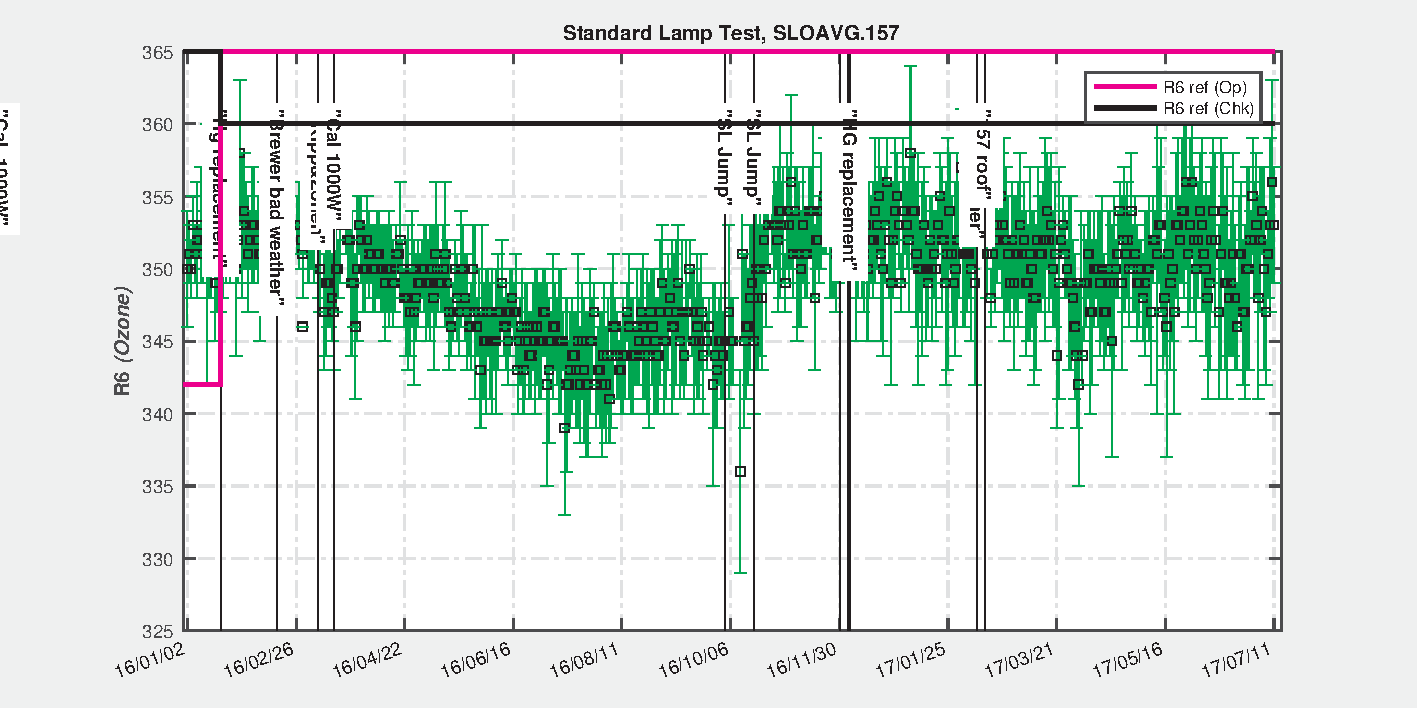
\includegraphics[width=\textwidth]{B_157_SLAVG_R6.pdf}
   \label{fig:SL_events}
   \caption{SL record and events analyzed}
\end{sidewaysfigure}

 
 \begin{sidewaystable}[h]

    % \IfFileExists{../tables/table_avg_185.tex}  % hacer una macro con esto
    %   {\resizebox{1.25\textwidth}{!}{
\begin{tabular}{lccccccccccccccc}
\toprule
&\textbf{"IZO"}&\textbf{"PTB"}&\textbf{"IZO"}&\textbf{Mantenimiento Kipp�zonen}&\textbf{" Arosa-Davos"}&\textbf{"Arosa-Davos 2016"}&\textbf{ATMOZ campaing}&\textbf{"Arduino Installed/ heater system broken"}&\textbf{"185 roof"}&\textbf{"Heater is working"}&\textbf{"Brewer at Marina/Germany"}&\textbf{"185 roof"}&\textbf{"Kipp\\&Zonnen.New filters 3\\&4. UV difuser"}&\textbf{"Brewer at Huelva 2017"}&\textbf{"Brewer at Iza\�a"}\\\midrule
\textbf{R6}&324.5&322&327.1667&330.7347&329.5882&329.2037&331.5&333.6429&333.5&333.25&334&333.8&335.4194&335.1538&335.2424\\\midrule
\textbf{std}&1.118&21&1.4162&1.2084&1.331&1.3524&1.2277&1.231&1.9365&1.199&0&1.3266&0.87156&1.0263&0.69763\\\midrule
\textbf{R5}&475&470.5&482.1&484.3367&482.7647&482.537&485.7&488.0714&488.875&489.125&491&490.6667&494.3548&495.6154&494.4848\\\midrule
\textbf{std}&2.2361&41.5&2.9479&1.6839&2.5095&2.3782&2.0096&1.8309&2.4463&2.0425&0&2.2706&1.6471&1.4956&1.1314\\\midrule
\textbf{N}&4&2&30&98&17&54&70&14&16&32&1&15&62&13&33\\\midrule
\textbf{DT high}&29.8054&30.5183&29.0571&29.2888&30.5521&29.057&28.954&29.2934&28.8151&29.9445&29.8955&28.5798&28.9554&29.9244&29.0479\\\midrule
\textbf{std}&0.35105&0.31361&1.5835&0.72011&0.27617&0.4771&0.69249&0.66428&0.82854&0.56516&0.3615&0.72406&0.58375&0.3229&0.3397\\\midrule
\textbf{DT low}&29.0076&28.3091&27.6736&28.6469&30.1045&28.3052&28.3469&28.3066&28.4774&29.0223&28.329&28.0128&28.4942&29.0894&28.454\\\midrule
\textbf{std}&0.97496&1.8212&2.4185&1.4078&1.3103&1.2032&1.3584&1.7099&1.9448&1.0968&0.946&0.8614&1.2896&1.2095&0.9483\\\midrule
\textbf{N}&5&7&30&98&19&53&71&14&16&31&2&16&62&15&35\\\midrule
\textbf{HT}&1120.68&1120.68&1119.9213&1118.7002&1118.72&1118.6474&1119.3273&1086.39&1116.5156&1118.7832&1120.68&1119.7576&1119.7467&1120.5493&1120.456\\\midrule
\textbf{std}&0&1.2396&0.95469&0.59063&0&0.84032&0.90637&1.2285&4.8428&0.60644&0.76878&0.9783&0.97889&0.48891&0.77999\\\midrule
\textbf{+5V}&5.38&5.363&5.3752&5.3752&5.3647&5.3613&5.3786&5.2993&5.375&5.3784&5.3562&5.3747&5.3779&5.3667&5.3649\\\midrule
\textbf{std}&0&0.012689&0.0056059&0.0070157&0.018459&0.021521&0.007179&0.0045737&0.014142&0.0057343&0.015951&0.0049913&0.0050893&0.012996&0.016453\\\midrule
\textbf{SL current}&1.69&1.678&1.6894&1.6875&1.6832&1.6843&1.6855&1.65&1.7738&1.6861&1.6754&1.6841&1.6843&1.678&1.6863\\\midrule
\textbf{std}&0&0.006&0.0024567&0.0043446&0.0046483&0.0049448&0.0052511&2.2204e-16&0.22539&0.0048709&0.0049852&0.0049215&0.0052597&0.004&0.0048319\\\midrule
\textbf{N}&5&10&31&99&19&54&71&14&16&31&13&17&63&15&35\\\midrule
\textbf{RS0}&1.0003&0.99953&0.99992&0.99971&0.99961&0.99963&0.99968&0.99978&0.99926&0.99983&0.99985&0.99995&0.99954&0.99963&0.99969\\\midrule
\textbf{std}&0.00071722&0.00081377&0.00087002&0.00073202&0.00098563&0.00059689&0.00071335&0.00047985&0.0006918&0.00072965&0.00035&0.0010416&0.00069127&0.00053225&0.0007926\\\midrule
\textbf{RS1}&0.99978&0.99927&0.99961&0.9996&0.99964&0.9997&0.99952&0.99932&0.99953&0.9998&0.99865&0.99969&0.99967&0.99957&0.99952\\\midrule
\textbf{std}&0.0003544&0.00078457&0.0007256&0.00065418&0.00065229&0.00072904&0.00069701&0.00066995&0.00093723&0.00072933&0.00135&0.00053906&0.00068636&0.00041226&0.00069795\\\midrule
\textbf{RS2}&0.9995&0.99983&0.99964&0.99981&0.99965&0.99982&0.99981&0.99972&0.99971&0.99981&0.99995&1.0001&0.9999&0.99959&0.99971\\\midrule
\textbf{std}&0.00086718&0.000836&0.00074503&0.00059413&0.00061075&0.00056414&0.00070756&0.00046626&0.00061935&0.00080416&0.00015&0.00063934&0.0007129&0.00061152&0.00058892\\\midrule
\textbf{RS3}&1.0003&1.0001&0.9997&0.99995&0.99987&0.9998&0.99994&0.99979&0.99982&0.99979&1.0003&0.99976&0.9998&0.99961&0.99997\\\midrule
\textbf{std}&0.00063435&0.0005252&0.00055527&0.0005457&0.00063912&0.00056984&0.00059484&0.00042234&0.00053411&0.00047366&0.0003&0.00061641&0.00068403&0.00060494&0.00059873\\\midrule
\textbf{RS4}&0.99936&0.9997&0.99989&0.99989&1.0002&1.0001&0.99998&0.99983&0.9998&0.99998&1.0001&0.99962&1&1.0001&0.99999\\\midrule
\textbf{std}&0.00034409&0.00041633&0.00054059&0.00053402&0.00042719&0.00051763&0.00054608&0.00071955&0.00036572&0.00053322&0.0002&0.00055621&0.00059896&0.00050711&0.0004021\\\midrule
\textbf{RS5}&1.0001&0.99978&1.0001&1.0001&1&1.0001&1.0001&0.99982&1.0001&1.0001&1.0001&1.0001&1&1.0002&1.0001\\\midrule
\textbf{std}&0.0003763&0.00038042&0.00052945&0.00053445&0.00051815&0.00050745&0.00042304&0.00045226&0.00057632&0.0005979&0.0003&0.00061234&0.0005295&0.00051208&0.00057445\\\midrule
\textbf{RS6}&1.0001&0.99977&1.0001&1.0001&1.0001&1.0001&1.0001&1.0001&0.99992&1.0001&1&1.0001&1.0001&1.0001&1.0001\\\midrule
\textbf{std}&0.00013565&0.00026874&0.00041692&0.00051544&0.00045592&0.00066988&0.00057739&0.00030573&0.00045169&0.00046849&0.00045&0.00038161&0.00035909&0.00039632&0.00039785\\\midrule
\textbf{N}&5&6&30&98&19&53&71&14&16&31&2&16&62&15&35\\
\bottomrule
\end{tabular}
}}
    %  {\resizebox{1.25\textwidth}{!}{
\begin{tabular}{lccccccccccccccc}
\toprule
&\textbf{"IZO"}&\textbf{"PTB"}&\textbf{"IZO"}&\textbf{Mantenimiento Kipp�zonen}&\textbf{" Arosa-Davos"}&\textbf{"Arosa-Davos 2016"}&\textbf{ATMOZ campaing}&\textbf{"Arduino Installed/ heater system broken"}&\textbf{"185 roof"}&\textbf{"Heater is working"}&\textbf{"Brewer at Marina/Germany"}&\textbf{"185 roof"}&\textbf{"Kipp\\&Zonnen.New filters 3\\&4. UV difuser"}&\textbf{"Brewer at Huelva 2017"}&\textbf{"Brewer at Iza\�a"}\\\midrule
\textbf{R6}&324.5&322&327.1667&330.7347&329.5882&329.2037&331.5&333.6429&333.5&333.25&334&333.8&335.4194&335.1538&335.2424\\\midrule
\textbf{std}&1.118&21&1.4162&1.2084&1.331&1.3524&1.2277&1.231&1.9365&1.199&0&1.3266&0.87156&1.0263&0.69763\\\midrule
\textbf{R5}&475&470.5&482.1&484.3367&482.7647&482.537&485.7&488.0714&488.875&489.125&491&490.6667&494.3548&495.6154&494.4848\\\midrule
\textbf{std}&2.2361&41.5&2.9479&1.6839&2.5095&2.3782&2.0096&1.8309&2.4463&2.0425&0&2.2706&1.6471&1.4956&1.1314\\\midrule
\textbf{N}&4&2&30&98&17&54&70&14&16&32&1&15&62&13&33\\\midrule
\textbf{DT high}&29.8054&30.5183&29.0571&29.2888&30.5521&29.057&28.954&29.2934&28.8151&29.9445&29.8955&28.5798&28.9554&29.9244&29.0479\\\midrule
\textbf{std}&0.35105&0.31361&1.5835&0.72011&0.27617&0.4771&0.69249&0.66428&0.82854&0.56516&0.3615&0.72406&0.58375&0.3229&0.3397\\\midrule
\textbf{DT low}&29.0076&28.3091&27.6736&28.6469&30.1045&28.3052&28.3469&28.3066&28.4774&29.0223&28.329&28.0128&28.4942&29.0894&28.454\\\midrule
\textbf{std}&0.97496&1.8212&2.4185&1.4078&1.3103&1.2032&1.3584&1.7099&1.9448&1.0968&0.946&0.8614&1.2896&1.2095&0.9483\\\midrule
\textbf{N}&5&7&30&98&19&53&71&14&16&31&2&16&62&15&35\\\midrule
\textbf{HT}&1120.68&1120.68&1119.9213&1118.7002&1118.72&1118.6474&1119.3273&1086.39&1116.5156&1118.7832&1120.68&1119.7576&1119.7467&1120.5493&1120.456\\\midrule
\textbf{std}&0&1.2396&0.95469&0.59063&0&0.84032&0.90637&1.2285&4.8428&0.60644&0.76878&0.9783&0.97889&0.48891&0.77999\\\midrule
\textbf{+5V}&5.38&5.363&5.3752&5.3752&5.3647&5.3613&5.3786&5.2993&5.375&5.3784&5.3562&5.3747&5.3779&5.3667&5.3649\\\midrule
\textbf{std}&0&0.012689&0.0056059&0.0070157&0.018459&0.021521&0.007179&0.0045737&0.014142&0.0057343&0.015951&0.0049913&0.0050893&0.012996&0.016453\\\midrule
\textbf{SL current}&1.69&1.678&1.6894&1.6875&1.6832&1.6843&1.6855&1.65&1.7738&1.6861&1.6754&1.6841&1.6843&1.678&1.6863\\\midrule
\textbf{std}&0&0.006&0.0024567&0.0043446&0.0046483&0.0049448&0.0052511&2.2204e-16&0.22539&0.0048709&0.0049852&0.0049215&0.0052597&0.004&0.0048319\\\midrule
\textbf{N}&5&10&31&99&19&54&71&14&16&31&13&17&63&15&35\\\midrule
\textbf{RS0}&1.0003&0.99953&0.99992&0.99971&0.99961&0.99963&0.99968&0.99978&0.99926&0.99983&0.99985&0.99995&0.99954&0.99963&0.99969\\\midrule
\textbf{std}&0.00071722&0.00081377&0.00087002&0.00073202&0.00098563&0.00059689&0.00071335&0.00047985&0.0006918&0.00072965&0.00035&0.0010416&0.00069127&0.00053225&0.0007926\\\midrule
\textbf{RS1}&0.99978&0.99927&0.99961&0.9996&0.99964&0.9997&0.99952&0.99932&0.99953&0.9998&0.99865&0.99969&0.99967&0.99957&0.99952\\\midrule
\textbf{std}&0.0003544&0.00078457&0.0007256&0.00065418&0.00065229&0.00072904&0.00069701&0.00066995&0.00093723&0.00072933&0.00135&0.00053906&0.00068636&0.00041226&0.00069795\\\midrule
\textbf{RS2}&0.9995&0.99983&0.99964&0.99981&0.99965&0.99982&0.99981&0.99972&0.99971&0.99981&0.99995&1.0001&0.9999&0.99959&0.99971\\\midrule
\textbf{std}&0.00086718&0.000836&0.00074503&0.00059413&0.00061075&0.00056414&0.00070756&0.00046626&0.00061935&0.00080416&0.00015&0.00063934&0.0007129&0.00061152&0.00058892\\\midrule
\textbf{RS3}&1.0003&1.0001&0.9997&0.99995&0.99987&0.9998&0.99994&0.99979&0.99982&0.99979&1.0003&0.99976&0.9998&0.99961&0.99997\\\midrule
\textbf{std}&0.00063435&0.0005252&0.00055527&0.0005457&0.00063912&0.00056984&0.00059484&0.00042234&0.00053411&0.00047366&0.0003&0.00061641&0.00068403&0.00060494&0.00059873\\\midrule
\textbf{RS4}&0.99936&0.9997&0.99989&0.99989&1.0002&1.0001&0.99998&0.99983&0.9998&0.99998&1.0001&0.99962&1&1.0001&0.99999\\\midrule
\textbf{std}&0.00034409&0.00041633&0.00054059&0.00053402&0.00042719&0.00051763&0.00054608&0.00071955&0.00036572&0.00053322&0.0002&0.00055621&0.00059896&0.00050711&0.0004021\\\midrule
\textbf{RS5}&1.0001&0.99978&1.0001&1.0001&1&1.0001&1.0001&0.99982&1.0001&1.0001&1.0001&1.0001&1&1.0002&1.0001\\\midrule
\textbf{std}&0.0003763&0.00038042&0.00052945&0.00053445&0.00051815&0.00050745&0.00042304&0.00045226&0.00057632&0.0005979&0.0003&0.00061234&0.0005295&0.00051208&0.00057445\\\midrule
\textbf{RS6}&1.0001&0.99977&1.0001&1.0001&1.0001&1.0001&1.0001&1.0001&0.99992&1.0001&1&1.0001&1.0001&1.0001&1.0001\\\midrule
\textbf{std}&0.00013565&0.00026874&0.00041692&0.00051544&0.00045592&0.00066988&0.00057739&0.00030573&0.00045169&0.00046849&0.00045&0.00038161&0.00035909&0.00039632&0.00039785\\\midrule
\textbf{N}&5&6&30&98&19&53&71&14&16&31&2&16&62&15&35\\
\bottomrule
\end{tabular}
}}
 \end{sidewaystable}
 
\subsection{Brewer \#185: temperature dependence} 
Due to the ICF introduced in the brewer is not the current ICF, the experimental R6 values must be calculated from raw counts. This also permits studying the temperature dependence of the brewer. As it is shown in the Figure 2, the current TC are not good (more 5 units/10ºC) and, hence, a new set the TC has been calculated (alternative configuration).  The new set reduce significantly this dependence.

\subsection{Brewer \#157: Dead Time} 
On the other hand, as it is shown in the figure 3, the Dead Time presents a mean value stable and closed to the operative value (26ns). Although, from October 2016, the DT values are noisy with large deviation between them.


\begin{figure}[bh]

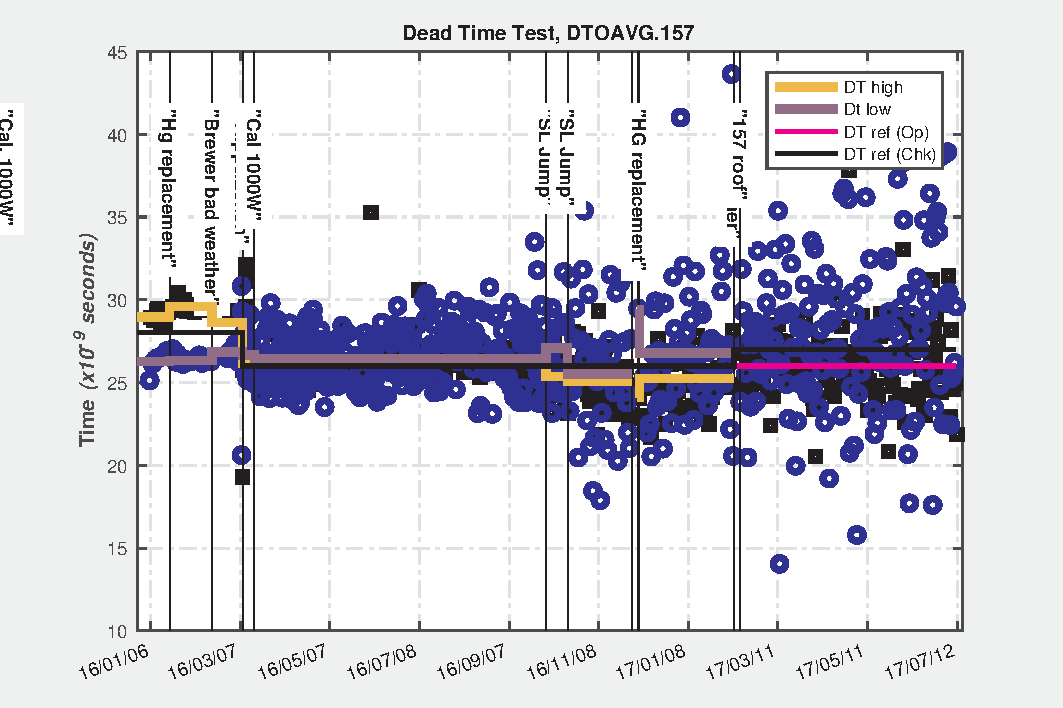
\includegraphics[width=\textwidth]{B_157_DTAVG.pdf}
\label{fig:DT_comp}
\caption{DT Record durig reporting period}
\end{figure}
 
 
\subsection{Brewer \#185: Filter} 

No filter dependence.
 \begin{table}[h]
\IfFileExists{../tables/table_fi_157.tex}  % hacer una macro con esto
        {\resizebox{0.9\textwidth}{!}{
\begin{tabular}{lcc}
\toprule
&\textbf{"Chg Hg"}&\textbf{"Fix Power Suply "}\\\midrule
\textbf{F1 corr}&-1.132&NaN\\\midrule
\textbf{se}&0.67906&NaN\\\midrule
\textbf{F2 corr}&-4.1347&NaN\\\midrule
\textbf{se}&0.68213&NaN\\\midrule
\textbf{F3 corr}&-5.9861&NaN\\\midrule
\textbf{se}&0.64288&NaN\\\midrule
\textbf{F4 corr}&3.456&NaN\\\midrule
\textbf{se}&0.84202&NaN\\\midrule
\textbf{F5 corr}&7.6678&NaN\\\midrule
\textbf{se}&2.5688&NaN\\\midrule
\textbf{N}&992&NaN\\
\bottomrule
\end{tabular}
}}
       {\resizebox{0.9\textwidth}{!}{
\begin{tabular}{lcc}
\toprule
&\textbf{"Chg Hg"}&\textbf{"Fix Power Suply "}\\\midrule
\textbf{F1 corr}&-1.132&NaN\\\midrule
\textbf{se}&0.67906&NaN\\\midrule
\textbf{F2 corr}&-4.1347&NaN\\\midrule
\textbf{se}&0.68213&NaN\\\midrule
\textbf{F3 corr}&-5.9861&NaN\\\midrule
\textbf{se}&0.64288&NaN\\\midrule
\textbf{F4 corr}&3.456&NaN\\\midrule
\textbf{se}&0.84202&NaN\\\midrule
\textbf{F5 corr}&7.6678&NaN\\\midrule
\textbf{se}&2.5688&NaN\\\midrule
\textbf{N}&992&NaN\\
\bottomrule
\end{tabular}
}}
\end{table}


\end{document}